%\documentclass[twoside,9pt]{extarticle}
\documentclass[12pt,twoside]{article}
\usepackage{jmlda}

%\usepackage{listings}
%\usepackage{caption}
%\DeclareCaptionFont{white}{\color{white}}
%\DeclareCaptionFormat{listing}{\colorbox{gray}{\parbox{\textwidth}{#1#2#3}}}
%\captionsetup[lstlisting]{format=listing,labelfont=white,textfont=white}
%%\NOREVIEWERNOTES

% Здесь можно определять собственные команды, они будут действовать только внутри статьи:
\newenvironment{coderes}%
    {\medskip\tabcolsep=0pt\begin{tabular}{>{\small}l@{\quad}|@{\quad}l}}%
    {\end{tabular}\medskip}

\begin{document}

\title{Рекомендации по подготовке статей к публикации}
\author{Редколлегия журнала}
\email{info@jmlda.org}
\organization{Москва, Вычислительный Центр им.\;А.\,А.\,Дородницына РАН}

\abstract{
    Данный документ содержит рисунки и рекомендации по~подготовке сборника статей в~издательской системе \LaTeXe\
    с~использованием стилевого файла \texttt{jmlda.sty}. Описанная здесь технология применялась при~подготовке всероссийской конференции <<Математические методы распознавания образов>> и международной конференции <<Интеллектуализация обработки информации>> и разработана К.\,В.~Воронцовым.
%    Документ распространяется свободно через сайт журнала \url{jmlda.org}

\bigskip
\textbf{Ключевые слова}: \emph {jmlda, оформление статей}.}
\titleEng{Style guide for authors}
\authorEng{JMLDA editorial board}
\organizationEng{Moscow, CCAS~RAS}
\abstractEng{
    This document explains how to prepare papers using \LaTeXe\
    typesetting system and style file \texttt{jmlda.sty}.

    \bigskip
    \textbf{Keywords}: \emph{jmlda, preparing papers using \LaTeXe\ }.}
\maketitle
%\linenumbers
Работу над статьёй удобно начинать с~редактирования
файла-образца \verb'jmlda-example.tex'.

Исходный текст статьи в~формате \LaTeXe\
можно набирать в~любом текстовом редакторе.

Текст статьи должен начинаться со~строк
{\small\begin{verbatim}
   \documentclass[twoside]{article}
   \usepackage{jmlda}
   \begin{document}
\end{verbatim}}

Команда \verb'\usepackage' подключает стилевой файл \verb'jmlda.sty',
который должен располагаться в~той~же директории, что и~сама статья.



Если статья написана по-английски, то это надо указать явно,
сразу после \verb|\begin{document}|
(иначе не~включатся английские переносы слов):
{\small\begin{verbatim}
   \English
\end{verbatim}}

Затем формируется заголовок статьи, включая ссылку на~грант и~аннотацию:
{\small\begin{verbatim}
   \title[Краткое название]{Полное название}
   \author{Фамилия~И.\,О., Фамилия~И.\,О.}
   \email{author@site.ru}
   \organization{Город, Организация}
   \abstract{Данная статья посвящена...}
   \thanks{Ссылка на грант.}
\end{verbatim}}

Если статья написана по"=русски, то~нужно задать второй заголовок
с~переводом названия, фамилий авторов и~аннотации на~английский язык:
{\small\begin{verbatim}
   \titleEng[Short title]{Full title}
   \authorEng{Author~N.\,S., Author~N.\,S.}
   \organizationEng{Organization, City, Country}
   \abstractEng{This paper...}
\end{verbatim}}

Если статья написана по"~английски, то~можно задать второй заголовок
с~переводом названия, фамилий авторов и~аннотации на~русский язык:
{\small\begin{verbatim}
   \titleRus[Краткое название]{Полное название}
   \authorRus{Фамилия~И.\,О., Фамилия~И.\,О.}
   \organizationRus{Город, Организация}
   \abstractRus{Данная статья посвящена...}
\end{verbatim}}

Все эти команды  могут идти в~произвольном порядке
и~должны завершаться командой
{\small\begin{verbatim}
   \maketitle
\end{verbatim}}

%Команды \verb|\email| и~\verb|\thanks|
%не имеют \mbox{Eng} и~\mbox{Rus} аналогов,
%и~указываются только в~основном заголовке.

Команды \verb|\title| и~\verb|\author|
могут иметь необязательный аргумент в~квадратных скобках \emph{перед} обязательным "---
это сокращённые версии названия и~списка авторов для колонтитулов.
Если колонтитул умещается в~одну строку, то~соответствующий необязательный аргумент не~нужен.

Кроме того, команда \verb'\author' может иметь необязательный аргумент в~квадратных скобках \emph{после} обязательного.
Он~указывается в~тех случаях, когда в~заголовок необходимо вывести дополнительную информацию, например об организациях:
{\small\begin{verbatim}
   \author{Автор~И.\,О., Соавтор~И.\,О.}
      [Автор~И.\,О.$^1$, Соавтор~И.\,О.$^2$]
   \organization{Москва, $^1$НИИ-X, $^2$НИИ-Y}
\end{verbatim}}

Иная расстановка инициалов, пробелов или запятых в~обязательном аргументе команды \verb'\author'
может приводить к~ошибкам в~оглавлении и~авторском указателе.

Ссылка на~грант(ы) оформляется как часть заголовка командой \verb'\thanks'
и~выводится в~виде сноски на~первой странице статьи.

Аннотация (не~более 10 строк) не~должна содержать ссылок, формул, таблиц, рисунков.

%После заголовка должна следовать аннотация:
%{\small\begin{verbatim}
%   \begin{abstract}
%      Вкратце: что за задача, и в чём результат.
%   \end{abstract}
%\end{verbatim}}
После команды \verb|\maketitle| необходимо включить нумерацию строк, для удобства общения автора с рецензентами. Для этого за командой \verb|\maketitle|
должна следовать команда
{\small\begin{verbatim}
   \linenumbers
\end{verbatim}}

Текст статьи можно разбивать на~разделы и~параграфы командами
{\small\begin{verbatim}
   \section{Название раздела}
   \paragraph{Название параграфа.}
\end{verbatim}}

Команды \verb'\subsection', \verb'\subparagraph' не~предусмотрены.
В~конце названий разделов точка не~ставится.
\mbox{Название} параграфа является частью первой строки абзаца;
если это целое предложение, то~точка ставится перед закрывающей фигурной скобкой.

\medskip
Статья должна заканчиваться командой
{\small\begin{verbatim}
   \end{document}
\end{verbatim}}

Каждая статья в~сборнике начинается с~новой страницы,
что позволяет сохранять заданное автором расположение материала на~страницах.
Убедительная просьба "--- не~использовать команды сокращения вертикальных промежутков
и~другие способы искусственного уплотнения текста.

%Работу над статьёй удобно начинать с~редактирования
%файла-образца \verb'jmlda-example.tex'.

\section{Стандартные средства \LaTeX'а}

Нет особых ограничений на~использование основных средств \LaTeX'а~%
\cite{VoronLatex,Goossens,Kotelnikov,Lvovsky}.
В~статью можно вставлять формулы, таблицы, списки, рисунки, сноски, и~т.\,д.
Определения ссылок \verb'\label'
и~команд \verb'\newcommand', \verb'\renewcommand'
действуют только внутри одной статьи;
конфликты с~чужими статьями исключены.

\paragraph{Стандартные пакеты,}%
подключённые в~стилевом файле \verb'jmlda.sty':
\verb'algorithm',
\verb'algorithmic',
\verb'amssymb',
\verb'amsmath',
\verb'array',
\verb'babel',
\verb'balance',
\verb'color',
\verb'epic',
\verb'euscript',
\verb'graphicx',
\verb'ifthen',
\verb'inputenc',
\verb'mathrsfs',
\verb'pb-diagram',
\verb'theorem',
\verb'subfig',
%\verb'upgreek',
\verb'url',
\verb'xy'.
Этими пакетами можно пользоваться, не~вызывая команду \verb'\usepackage'.
Желательно обходиться только этими пакетами.

\paragraph{Формулы}%
внутри текста, даже очень короткие,
необходимо окружать знаками доллара~\verb'$':

\begin{coderes}
    \verb'число $-3.14$' & число $-3.14$ --- верно\\
    \verb'число -3.14'   & число -3.14 --- неверно   \\
    \verb'объект~$x$'    & объект~$x$ --- верно    \\
    \verb'объект x'      & объект x --- неверно
\end{coderes}

Выключные формулы без номера окружаются скобками \verb'\[' и \verb'\]'.
Выключные формулы с~номером окружаются командами
\verb'\begin{equation}' и~\verb'\end{equation}'.
Команда \verb'\label{'\emph{name}\verb'}' между ними
задаёт метку формулы.
Русские буквы в~именах меток~\emph{name} не~допустимы.
Метка позволяет ссылаться на~формулу командой
\verb'\eqref{'\emph{name}\verb'}',
например команда \verb'\eqref{eqCases}' даёт~\eqref{eqCases}.

\begin{table}[t]%\small
    \caption{Подпись размещается над таблицей.}
    \label{TabExample}
    \centering\medskip%\tabcolsep=2pt%\small
    \begin{tabular}{lrrr}
    \headline
        Задача
            & \multicolumn{1}{c}{CCEL}
            & \multicolumn{1}{c}{boosting} \\
    \headline
        {\tt Cancer}
            & $\mathbf{3.46}  \pm 0.37$ (3.16)
            & $4.14 \pm 1.48$ \\
        {\tt German}
            & $\mathbf{25.78} \pm 0.65$ (1.74)
            & $29.48 \pm 0.93$ \\
        {\tt Hepatitis}
            & $18.38 \pm 1.43$ (2.87)
            & $19.90 \pm 1.80$ \\
    \hline
    \end{tabular}
\end{table}

\paragraph{Списки}%
оформляются стандартными окружениями \verb|enumerate| или \verb|itemize|.
В~стиле \verb|jmlda.sty| определено окружение \verb|enumerate*|
для списков, в~которых, согласно правилам русской пунктуации:
\begin{enumerate*}
\item
    номера отделяются скобкой;
\item
    пункты начинаются со~строчной буквы;
\item
    и~заканчиваются точкой с~запятой.
\end{enumerate*}
Этот список удобен для перечисления коротких пунктов, умещающихся в~одну строку.
Если пункты более длинные, то~лучше воспользоваться стандартным окружением \verb|enumerate|,
указав после \verb|\begin{enumerate}|
команду \verb|\afterlabel)|,
которая переопределит точку после номера на~скобку.

\paragraph{Таблицы}%
создаются окружением \verb'tabular'
и оформляются как плавающие с~помощью окружения  \verb'table'.
Желательно прижимать их~вверх страницы опцией~\verb|[t]| команды \verb'\begin{table}'.
Подпись делается \emph{над таблицей} командой \verb'\caption', см.~таблицу~\ref{TabExample}.
Команда \verb'\label', определяющая ссылку на~номер таблицы,
обязана идти после \verb'\caption'.
Если таблица не умещается по~ширине колонки,
то~можно уменьшить шрифт до~\verb'\small' или даже \verb'\footnotesize',
либо уменьшить интервалы между колонками:
\verb'\tabcolsep=2pt'.

\paragraph{Иллюстрации}%
должны быть подготовлены в~формате \verb'EPS'.
Для преобразования файлов формата \verb'PNG' или \verb'JPEG' в~\verb'EPS'
используйте утилиту \verb'bmeps', входящую в~пакет MiK\TeX.
Не~забудьте прислать графические файлы вместе с~\TeX-файлом!

Рисунки вставляются командой \verb|\includegraphics|,
желательно с~выравниванием по~ширине колонки: \verb|[width=\linewidth]|.
Если рисунок занимает по~высоте более 1--2~см,
то~он оформляется как плавающая иллюстрация \verb|{figure}|
с~прижатием вверх страницы опцией~~\verb|[t]|.
Подпись делается \emph{под рисунком} командой \verb|\caption|,
см.\,рис.\,\ref{TabExample}.

Практически все популярные пакеты рисуют графики с подписями, которые трудно читать на бумаге и на слайдах из-за малого размера шрифта. Шрифт на графиках (подписи осей и цифры на осях) должны быть такого же размера, что и основной текст.

\begin{figure}[h]
  \subfloat[Первый рисунок]{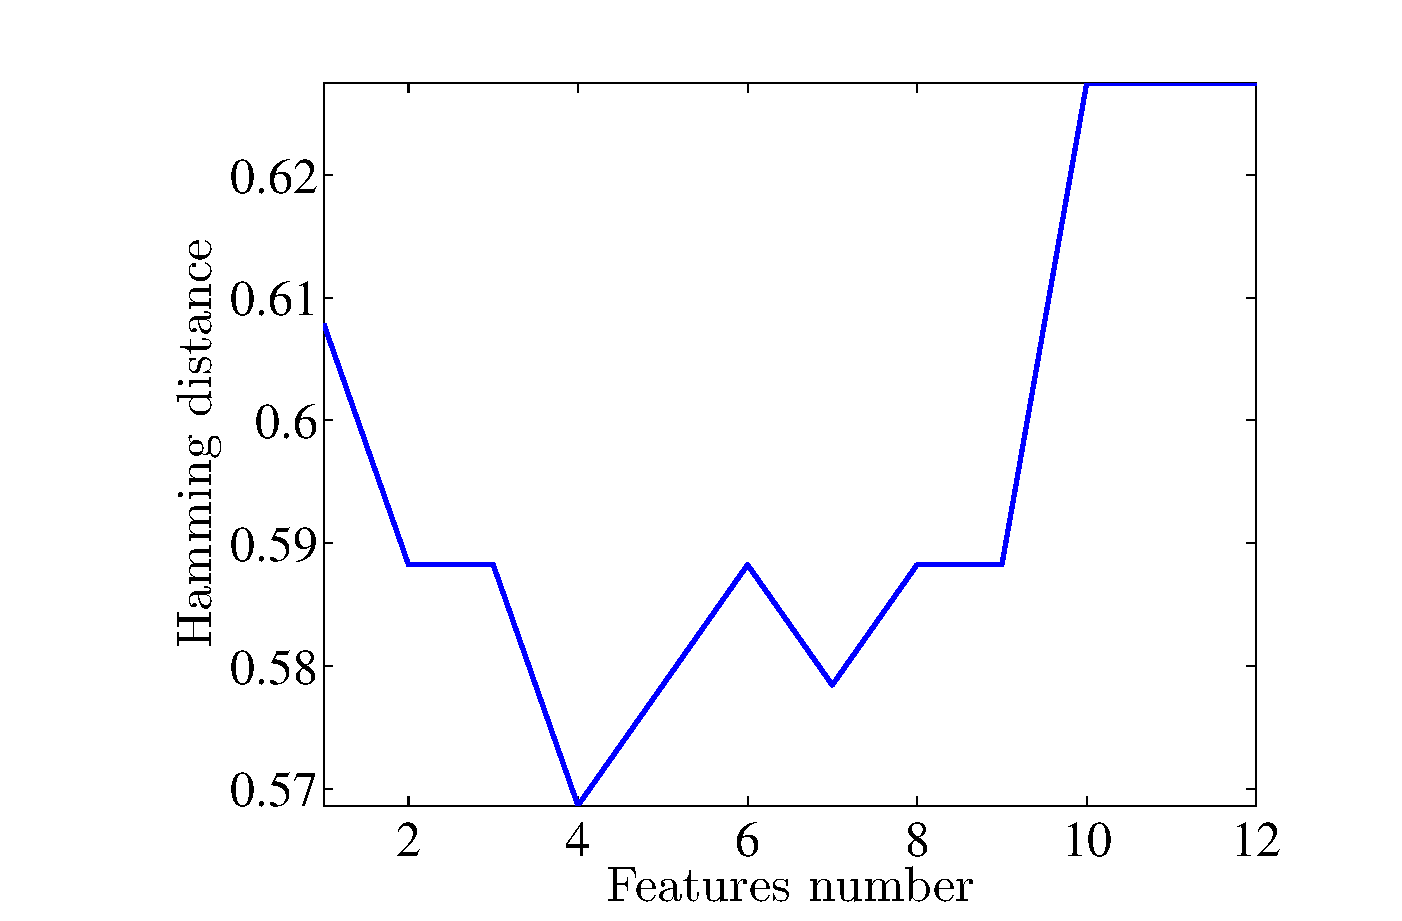
\includegraphics[width=0.5\textwidth]{figExample1}}
  \subfloat[Второй рисунок]{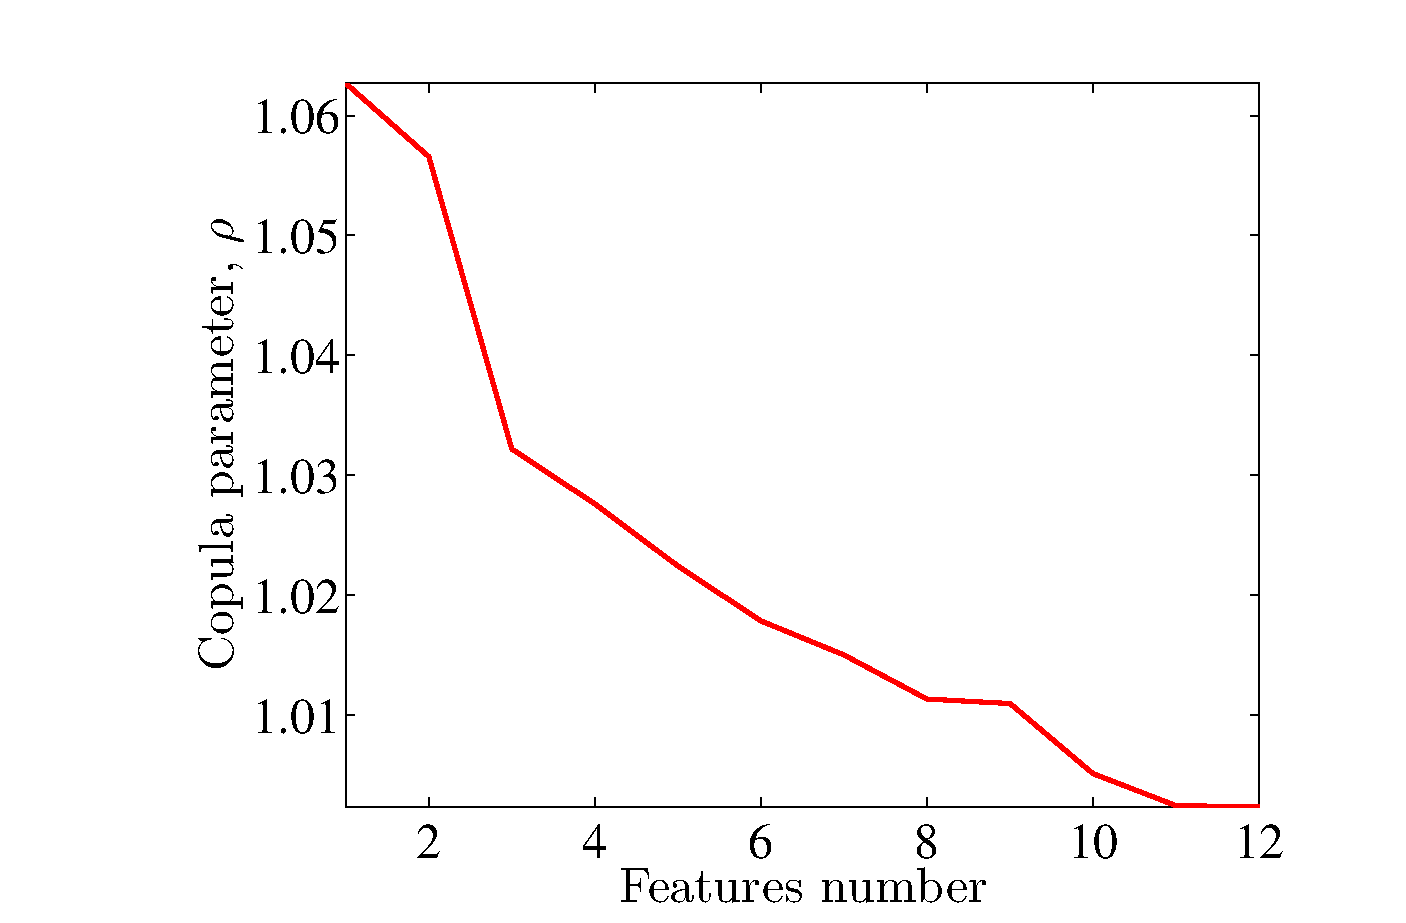
\includegraphics[width=0.5\textwidth]{figExample2}}\\
\caption{Подпись должна размещаться под рисунком. }
\label{fg:Example}
\end{figure}

При значительном количестве рисунков рекомендуется группировать иx в одном окружении \verb|figure|, как это сделано на рис.~\ref{fg:Example}.
Для этого используется пакет \verb|subfig|.

Определена команда \verb'\XYtext('$x$\verb','$y$\verb'){'\emph{text}\verb'}',
для надписей поверх рисунков.
%\TODO{До сих пор не решена проблема с~выводом надписи поверх изображения, а~не~под~ним.}
%Например, так сделана надпись <<$Q(\lambda)$>> на~рис.\,\ref{FigExample}.
Координаты левого нижнего угла надписи $(x,y)$ подбираются вручную
относительно правого нижнего угла рисунка.

\paragraph{Оформление иллюстраций} в популярных пакетах может быть выполнено следующим образом.
\begin{verbatim}
\begin{figure}[h]
  \subfloat[Первый рисунок]{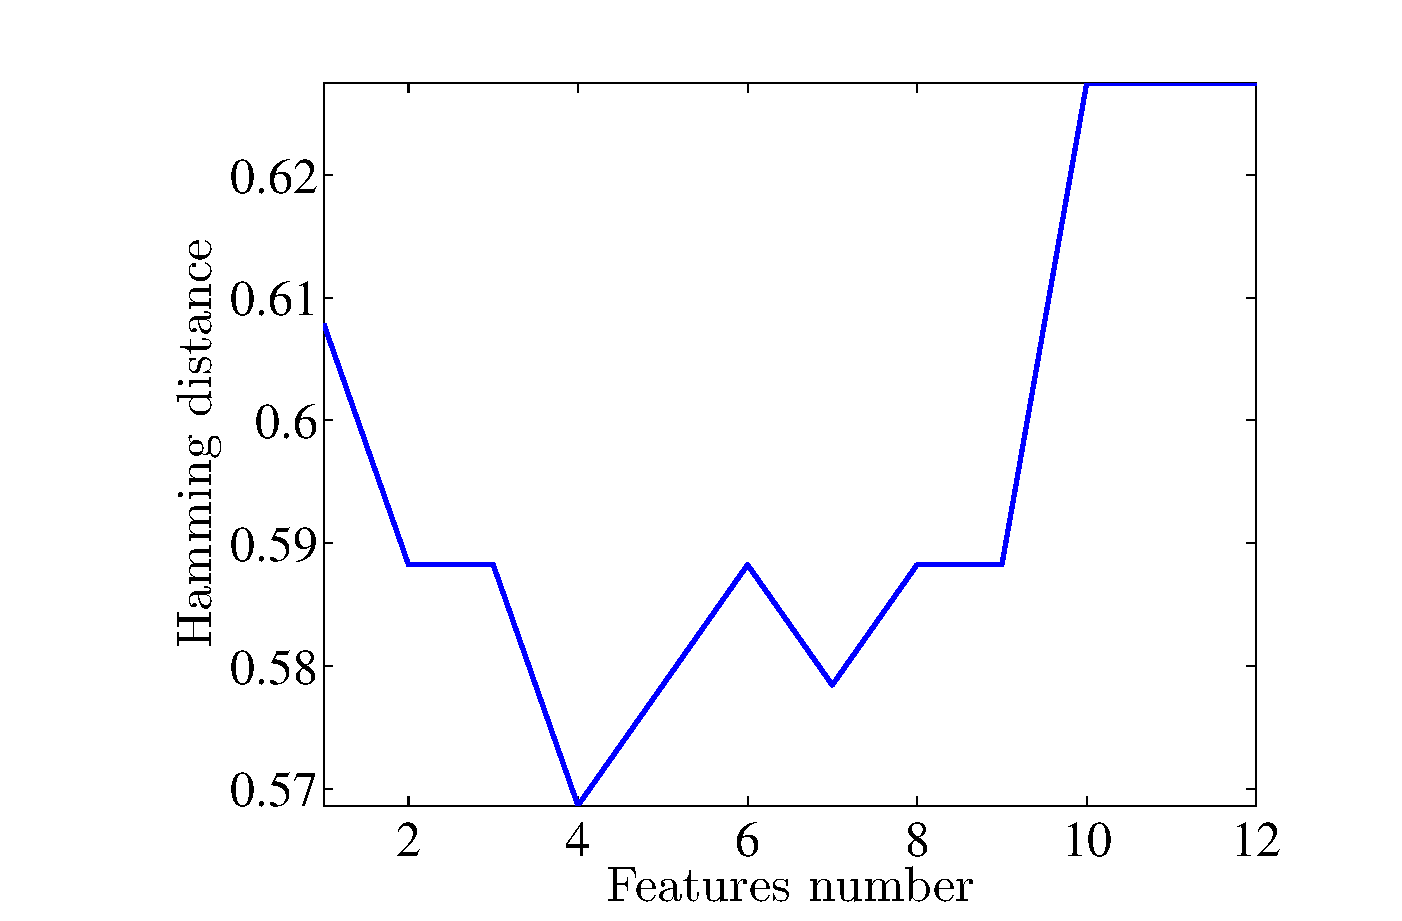
\includegraphics[width=0.5\textwidth]{figExample1}}
  \subfloat[Второй рисунок]{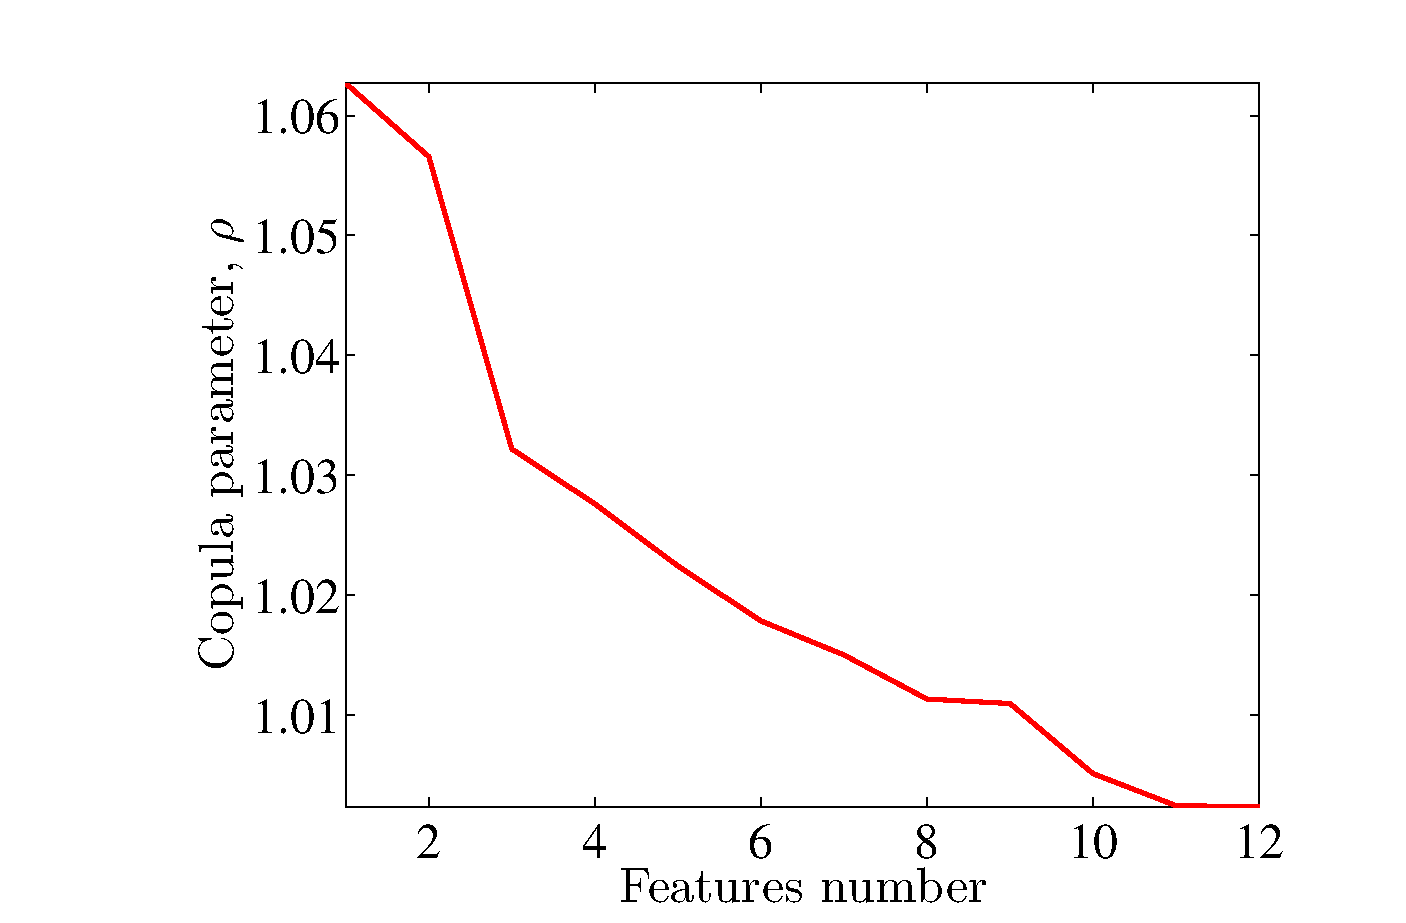
\includegraphics[width=0.5\textwidth]{figExample2}}\\
\caption{Подпись должна размещаться под рисунком. }
\label{fg:Example}
\end{figure}
\end{verbatim}

\paragraph{Советы по оформлению графиков в системе Matlab.}
\begin{itemize}
\item толщина линий равна двум;
\item заголовки осей пишутся с большой буквы;
\item необходимо включить интепретатор LaTeX для корректного отображения формул на осях;
\item заголовок графика отсутствует (чтобы не дублировать подпись графика в статье).
\item Рекомендуется сразу сохранять файлы в формате EPS и PNG.
\item Рекомендуемые параметры:
\begin{verbatim}
h = figure; hold('on');
plot(xi,y,'r-', 'Linewidth', 2);
plot(xi,y,'b.', 'MarkerSize', 12);
axis('tight');
xlabel('Time, $\xi$', 'FontSize', 24, 'FontName', 'Times', 'Interpreter','latex');
ylabel('Value, $y$', 'FontSize', 24, 'FontName', 'Times', 'Interpreter','latex');
set(gca, 'FontSize', 18, 'FontName', 'Times')
saveas(h,'ModelOne.eps', 'psc2');
saveas(h,'ModelOne.png', 'png');
\end{verbatim}
\end{itemize}

\paragraph{Оформление графиков в Inkscape.}

Inkscape~--- векторный графический редактор, удобный для создания технических иллюстраций.

Пример использования редактора.
\begin{enumerate}
\item Нарисовать изображение, используя, где необходимо, формулы в формате \LaTeX.
\item Сохранить изображение в формате eps, используя дополнительную опцию <<создать файл latex>>. На выходе сгенерируется два файла --- \verb|image.eps| и    \verb|image.eps_tex|, второй можно редактировать в tex-редакторе.
\item Вставить файл \verb|image.eps_tex| в код статьи, заменив при этом
\begin{verbatim}
\includegraphics[width=<desired width>]{image.eps}
\end{verbatim}
на
\begin{verbatim}
\def\svgwidth{<desired width>}
\input{image.eps_tex}
\end{verbatim}
\end{enumerate}

Пример использования редактора показан на рис.~\ref{fg:ExampleInk}. Слева показано исходное изображение в редакторе InkScape. Справа~--- полученное после компиляции в системе LaTeX изображение в формате eps.

\begin{figure}[h]
  \subfloat[Исходный рисунок в редакторе Inkscape]{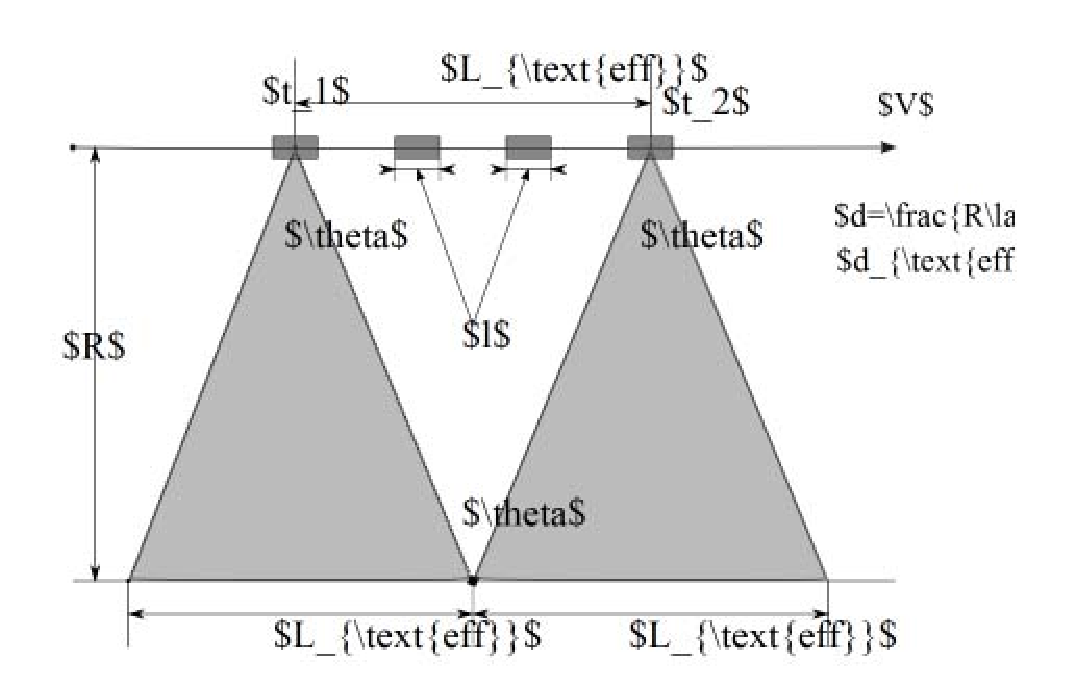
\includegraphics[width=0.5\textwidth]{figExample3}}
  \subfloat[Полученный рисунок]{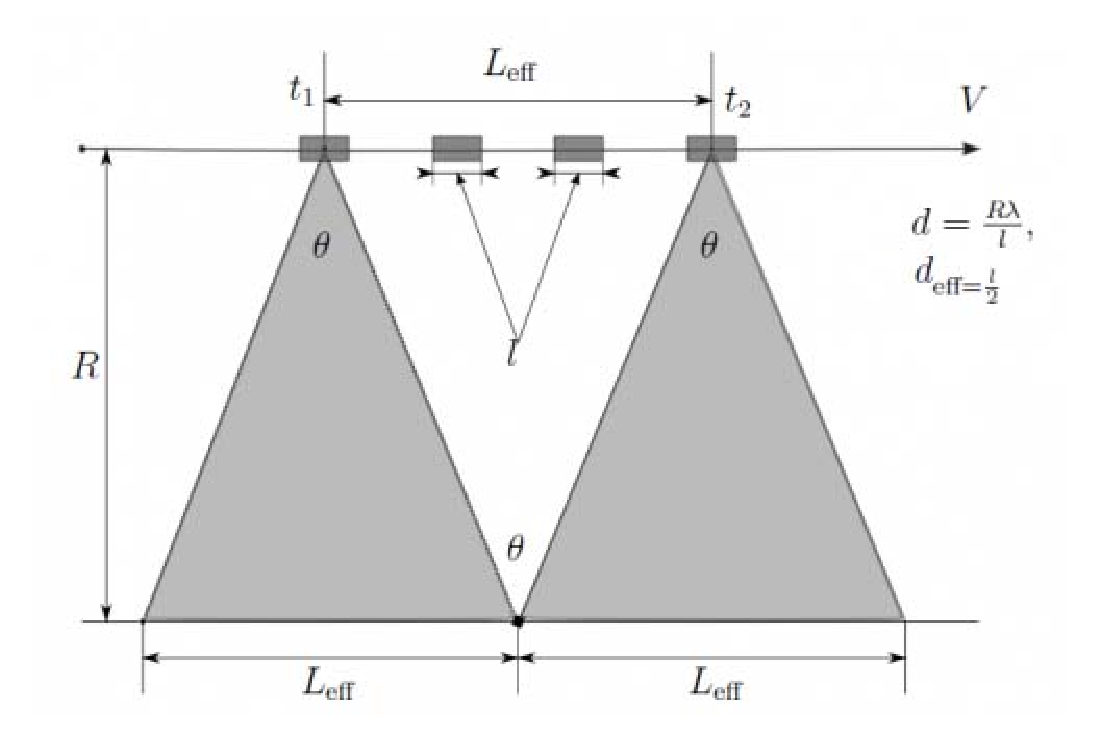
\includegraphics[width=0.5\textwidth]{figExample4}}\\
\caption{Пример использования редактора InkScape. }
\label{fg:ExampleInk}
\end{figure}

%Запрещается использовать пакеты, размещающие рисунки сбоку
%или влияющие на двухколоночный режим:
%\verb'multicol', \verb'floatfig', \verb'floatflt', и~т.\,п.
%Многие из~них работают некорректно:
%рисунок может перескочить в~конец раздела или вообще потеряться.

\paragraph{Сноски}%
делаются командой \verb'\footnote{'\emph{text}\verb'}'%
\footnote{Текст сноски указывается в~аргументе \emph{text}.}.

\paragraph{Список литературы}%
формируется окружением \verb'thebibliography'.
Каждая запись библиографии начинается командой
\verb'\bibitem{'\textit{name}\verb'}'.
Метка \textit{name} позволяет ссылаться на~данную запись командой
\verb'\cite{'\textit{name}\verb'}'.
В~ссылках разрешается указывать несколько меток через запятую:
\verb'\cite{'\textit{name$_1$,name$_2$}\verb'}'.
Новая команда \verb'\citenb' даёт ссылку без квадратных скобок, что позволяет делать интервалы;
например,
[\citenb{VoronLatex}--\citenb{Lvovsky}]
было получено так:
\verb'[\citenb{VoronLatex}--\citenb{Lvovsky}]'.
Русские буквы в~именах меток \textit{name} недопустимы.
Записи сортируются по авторам в~порядке русского, затем латинского алфавита.

Фамилии и~инициалы авторов выделяются командой \verb'\BibAuthor'.
Названия статей в~сборниках выделяются командой \verb'\BibTitle'.
Если публикация существует только в~электронном виде,
веб-ссылка даётся командой \verb'\BibUrl'.
В~остальном старайтесь придерживаться требований \mbox{ГОСТ~7.80-00}.
%\TODO{Перейти на~новый ГОСТ.}

\paragraph{Глобальные ссылки.}%
В~стиле \verb'jmlda.sty' определены команды
\verb'\globallabel',
\verb'\globalref',
\verb'\globalpageref',
позволяющие сослаться из~одной статьи на~любое место в~другой статье.
Это полные аналоги стандартных команд
\verb'\label',
\verb'\ref',
\verb'\pageref',
но~определяемые ими метки доступны во~всём сборнике.
Типичное применение этой возможности "---
указать в~библиографии диапазон страниц другой статьи <<в~настоящем сборнике>>:
{\small\begin{verbatim}
   C.\,\globalpageref{Kozlov:begin}--%
       \globalpageref{Kozlov:end}
\end{verbatim}}
Для каждой статьи в~сборнике по умолчанию определены две метки
\verb'\globallabel{'\textit{file}\verb':begin}' и~\verb'\globallabel{'\textit{file}\verb':end}',
где \textit{file} "--- имя tex-файла статьи, без указания расширения.

\paragraph{Ссылки на сайты} делаются командой \verb'\url'.
При вёрстке документа в~формате \verb'PDF' ссылки становятся активными,
хотя не~подчёркиваются и~не выделяются цветом.
Пример: \verb'\url{www.jmlda.org}'.

\section{Математические обозначения}

Следование приводимым ниже рекомендациям
способствует большему единообразию в~обозначениях
и~облегчает подготовку сборника.

Целочисленные интервалы обозначаются только как $1,\dots,n$.
Варианты $\overline{1,n}$ или $1,\dots,i,\dots,n$ или $1,2,\dots,n$
не~допустимы.
То~же относится к~векторам и~спискам переменных вида $x_1,\dots,x_n$.

В~качестве десятичного разделителя используется запятая:
в~формуле \verb|$3{,}14$|, в~тексте \verb|3,14|.

Числовые множества $\NN$, $\ZZ$, $\RR$, $\CC$
делаются командами \verb'\NN', \verb'\ZZ', \verb'\RR', \verb'\CC'.

В~стиле \verb'jmlda.sty' переопределены команды
\verb$\geq$,
\verb$\leq$,
\verb$\emptyset$,
\verb$\epsilon$,
\verb$\kappa$,
\verb$\phi$
математических символов
$\geq$,
$\leq$,
$\emptyset$,
$\epsilon$,
$\kappa$,
$\phi$.

Математические операторы $\lim$, $\inf$, $\sup$, $\min$, $\max$
переопределены так, что пределы всегда ставятся снизу, а~не~сбоку.

Определены математические операторы:
$\argmin$,
$\argmax$,
$\diag$,
$\sign$,
$\Tr$,
$\const$
командами
\verb$\argmin$,
\verb$\argmax$,
\verb$\diag$,
\verb$\sign$,
\verb$\Tr$,
\verb$\const$.

Команды \verb'\myop' и~\verb'\mylim' производят
новые операторы, не~предусмотренные \LaTeX'ом:

\begin{coderes}
    \verb'$\myop{Ker} f$'            & $\myop{Ker} f$ \\
    \verb'$A_{\myop{Ker} f}$'        & $A_{\myop{Ker} f}$ \\
    \verb'$\myop{Hom}_\Phi(A,B)$'    & $\myop{Hom}_\Phi(A,B)$ \\
    \verb'$\mylim{Hom}_\Phi(A,B)$  ' & $\mylim{Hom}_\Phi(A,B)$
\end{coderes}

Для выделения векторных и~матричных величин прямым жирным шрифтом
предусмотрена команда \verb'\vec{'\textit{формула}\verb'}'.

\paragraph{Линейная алгебра:}
\nopagebreak

\begin{coderes}
    \verb'$\rank A$'                 & $\rank A$ \\
    \verb'$\Tr A$'                   & $\Tr A$ \\
    \verb'$\diag (d_1,\dots,d_n)$'   & $\diag (d_1,\dots,d_n)$ \\
    \verb'$A\T$'                     & $A\T$ \\
    \verb'$u\T F\T F u$'             & $u\T F\T F u$ \\
    \verb'$\vec x$'                  & $\vec x$ \\
    \verb'$\Omega \neq \vec\Omega$'  & $\Omega \neq \vec\Omega$ \\
    \verb'$e^{-\vec{x\T\Sigma x}}$ ' & $e^{-\vec{x\T\Sigma x}}$ (верно)\\
    \verb'$e^{-x\T\Sigma x}$'        & $e^{-x\T\Sigma x}$ (неверно)
\end{coderes}

\paragraph{Теория вероятностей:}
\nopagebreak

\begin{coderes}
    \verb'$\Prob\{x\colon x\in A\}$' & $\Prob\{x\colon x\in A\}$ \\
    \verb'$\Expect \xi$'             & $\Expect \xi$ \\
    \verb'$\Var \xi$'                & $\Var \xi$ \\
    \verb'$\Normal(\mu,\Sigma)$'     & $\Normal(\mu,\Sigma)$ \\
    \verb'$p(x\cond y)$'             & $p(x\cond y)$
\end{coderes}

В~условных вероятностях команда \verb'\cond'
даёт правильные пробелы вокруг вертикальной черты.

\paragraph{Теория вычислительной сложности:}
\nopagebreak

\begin{coderes}
    \verb'$\P$                     ' & $\P$ \\
    \verb'$\NP$'      & $\NP$ \\
    \verb'$\DTIME$'   & $\DTIME$ \\
    \verb'$\MaxSNP$'  & $\MaxSNP$ \\
    \verb'$\Apx$'     & $\Apx$ \\
    \verb'$\PC$'      & $\PC$ \\
    \verb'$\MinPC$'   & $\MinPC$ \\
    \verb'$\threeSAT$'& $\threeSAT$ \\
    \verb'$\GapSAT$'  & $\GapSAT$
\end{coderes}

Легко определять собственные такие команды для новых классов сложности и~задач,
например, класс~\NP\ и задача \MinPC\ были определены так:
{\small\begin{verbatim}
   \def\NP{\CCfont{NP}}
   \def\MinPC{\CPfont{MinPC}}
\end{verbatim}}

Все эти команды могут употребляться как внутри формул, так и~непосредственно в~тексте.

Для оформления условных конструкций пользуйтесь стандартным окружением \verb'cases'.
Текст внутри формул выводится командой \verb'\text':
\begin{equation}\label{eqCases}
    y(x,\alpha) = \begin{cases}
        -1, & \text{если } f(x,\alpha)<0;  \\
        +1, & \text{если } f(x,\alpha)\geq 0.
    \end{cases}
\end{equation}
{\small\begin{verbatim}
   \begin{equation}\label{eqCases}
      y(x,\alpha) = \begin{cases}
         -1, & \text{если } f(x,\alpha)<0; \\
         +1, & \text{если } f(x,\alpha)\geq 0.
      \end{cases}
   \end{equation}
\end{verbatim}}

Чтобы размер скобок соответствовал размеру обрамляемой формулы,
пользуйтесь командами \verb'\left' и~\verb'\right'.
Однако в~простых случаях эти команды не~нужны и~только загромождают текст.
Лучше записать \verb'f(x_i)', чем \verb'f\left(x_i\right)'
"--- результат в~обоих случаях будет одинаков.

Для вставки матрицы в~строку текста
$
    \bigl(
    \begin{smallmatrix}
        a & b & c \\
        1 & 2 & 3
    \end{smallmatrix}
    \bigr)
$
используйте окружение \verb'smallmatrix'.
Все остальные способы дают некрасивый результат.

\paragraph{Окружения типа теорем.}
Следующие окружения выводят заключённый в~них текст {\slshape наклонным шрифтом}:
\verb'Def' или \verb'Definition' "--- Определение,
\verb'Theorem' "--- Теорема,
\verb'Lemma' "--- Лемма,
\verb'State' "--- Утверждение,
\verb'Corollary' "--- Следствие.

Следующие окружения выводят заключённый в~них текст обычным шрифтом:
\verb'Axiom' "--- Аксиома,
\verb'Problem' "--- Задача,
\verb'Example' "--- Пример,
\verb'Remark'~--- \mbox{Замечание,}
\verb'Hypothesis' "--- Гипотеза.


\section{Рекомендации по оформлению}

Придерживаясь следующих правил, авторы существенно облегчают подготовку сборника.
%Общие трудозатраты на~подготовку сборника существенно снижаются,
%если авторы придерживаются нескольких несложных правил, приведённых ниже.
%Авторам будет также полезно ознакомиться с~типичными ошибками,
%приведёнными в~рекомендациях корректорам и~рецензентам.

%По~возможности старайтесь вставлять рисунки и~таблицы как плавающие вверху страницы,
%и~только при острой необходимости вставляйте по~месту первого упоминания в~тексте.

\balance
\subparagraph{Некоторые правила типографики.}
Скобки всех видов набираются вплотную к тексту, который они окружают.
Знаки препинания набираются
слитно с~предшествующим текстом и~отдельно от~последующего.

Кавычки делаются в~русском тексте так: \verb'<<'\emph{текст}\verb'>>',
в~английском так: \verb|``|\emph{text}\verb|''|.
Использовать символ \verb'"' нельзя!

Многоточия в~тексте и~формулах делаются командой \verb'\dots'.

Тире отделяется от~предшествующего текста неразрывным пробелом:
\verb*'Знание~--- сила'.

В~длинных словах с~дефисом, таких, как <<счётно"=аддитивно>>,
дефис делается командой \verb'"=', иначе слово не~будет переноситься:
\verb'счётно"=аддитивно'.
Команда \verb'"~' запрещает перенос по~дефису:
$F$"~пре\-образование,
\verb'$F$"~пре\-образование'.
%В~английских текстах команды \verb'"=' и~\verb'"~' не~работают.

Неразрывный пробел~\verb'~' ставится
между коротким предлогом и~последующим словом,
\mbox{а~также} между очень короткой формулой и~связанным с~ней по~смыслу словом:
\verb'число~$N$ в~$k$~раз' \verb'больше, чем~$n$'.

Между идущими подряд формулами иногда нужен дополнительный пробел:

\begin{coderes}
    \verb'$a=1,b=2$'       & $a=1,b=2$ ~~~--- плохо \\
    \verb'$a=1$, $b=2$'    & $a=1$, $b=2$ ~~~--- получше \\
    \verb'$a=1$,\: $b=2$'  & $a=1$,\: $b=2$  ~~~--- хорошо \\
    \verb'$a=1$,\; $b=2$'  & $a=1$,\; $b=2$  ~~~--- хорошо
\end{coderes}

Иногда в~формуле надо убрать пробелы вокруг знака операции.
Например, если знак $\times$ используется не~как произведение,
а~для указания размеров матрицы или растрового изображения,
то~его лучше не~окружать пробелами:

\begin{coderes}
    \verb'$640\times 480$'  & $640\times 480$ ~~~--- плохо \\
    \verb'$640{\times}480$' & $640{\times}480$ ~~~--- хорошо
\end{coderes}

Дополнительный пробел \verb'\quad' рекомендуется вставлять
между длинными выражениями, идущими через запятую в~выключной формуле.

Короткий пробел \verb'\,' ставится
после знака номера: \verb|\No\,6|;
в~инициалах: \verb|И.\,В.\,Анов|;
в~сокращениях: \verb|т.\,к.|; \verb|т.\,е.|; \verb|и~т.\,д.|

Не~следует использовать жирный шрифт для выделения
\emph{важных слов} или \emph{терминов}.
Это делается командой \verb'\emph{'\emph{текст}\verb'}'.

\paragraph{Правила форматирования} исходного кода
облегчают его чтение и~работу над корректурой:
\begin{itemize}
\item
    начинайте каждое предложение с~новой строки;
\item
    набирайте отдельной строкой команды
    \verb'\begin', \verb'\end', \verb'$$', \verb'\[', \verb'\]',
    \verb'\section', \verb'\subsection', \verb'\paragraph'
    \verb'\item', \verb'\bibitem', \verb'\par', \verb'\label';
\item
    внутритекстовые формулы, за~исключением совсем коротких,
    набирайте отдельной строкой;
\item
    длинные описания формул разбивайте на строки;
    используйте табуляции для выделения вложенных скобок и~логически обособленных частей формул,
    как показано в~Примере~\ref{exExample}.
    %Это облегчает понимание и~правку формул в~\TeX-файлах.
\end{itemize}

\begin{Example}
\label{exExample}
    Форматирование сложной формулы:
    \begin{align*}
    R'_N(F)
        = \frac1N \sum_{i=1}^N
        \Bigl(
            & P(+1\cond x_i) C\bigl(+1,F(x_i)\bigr)
        +{} \\ {}+{}
            & P(-1\cond x_i) C\bigl(-1,F(x_i)\bigr)
        \Bigr).
    \end{align*}
\end{Example}
{\small\begin{verbatim}
    \begin{align*}
       R'_N(F)
       = \frac1N \sum_{i=1}^N
        \Bigl(
          & P(+1\cond x_i) C\bigl(+1,F(x_i)\bigr)
        +{} \\ {}+{}
          & P(-1\cond x_i) C\bigl(-1,F(x_i)\bigr)
        \Bigr).
    \end{align*}
\end{verbatim}}

Ссылка на грант(ы), если она есть, задаётся в~заголовке статьи
командой \verb'\thanks'.
В~конце статьи ссылаться на~грант уже не~нужно.

\paragraph{Оформление списка литературы.}
Порядок оформления позиций в списке литературы:
\begin{itemize}
\item[--] ссылка на статью в журнале: {\small\begin{verbatim}
\bibitem{author-and-co2007}
    \BibAuthor{Автор\;И.\,О., Соавтор\;И.\,О.}
    \BibTitle{Название статьи}~//
    \BibJournal{Название журнала}. 2007. Т.\,38, \No\,5.  С.\,54--62.
\end{verbatim}}

\medskip
\item[--] ссылка на статью в сборнике, доклад на конференции:
{\small\begin{verbatim}
\bibitem{author09first-word-of-the-title}
    \BibAuthor{Автор\;И.\,О.}
    \BibTitle{Название статьи}~//
    \BibJournal{Название конференции или сборника},
    Город:~Изд-во, 2009. С.\,5--6.
\end{verbatim}}

\medskip
\item[--] ссылка на книгу {\small\begin{verbatim}
\bibitem{myHandbook}
    \BibAuthor{Автор\;И.\,О.}
    Название книги.
    Город: Издательство, 2009. 314~с.
\end{verbatim}}

\medskip
\item[--] ссылка на электронный источник
{\small\begin{verbatim}
\bibitem{bibUsefulUrl}
    \BibUrl{www.site.ru}~---
    Название сайта. 2007.
\end{verbatim}}
\end{itemize}

\medskip
Пример оформления ссылки на английском
языке:{\small\begin{verbatim}
\bibitem{author09anyscience}
    \BibAuthor{Author\;N.}
    \BibTitle{Paper title}~//
    \BibJournal{10-th Int'l. Conf. on Anyscience}, 2009. Vol.\,11, No.\,1.  Pp.\,111--122.
\end{verbatim}}

\begin{thebibliography}{1}
\bibitem{VoronLatex}
    \BibAuthor{Воронцов~К.\,В.}
    \LaTeXe\ в~примерах.
    2006.~---
    \BibUrl{http://www.ccas.ru/voron/latex.html}.
\bibitem{Goossens}
    \BibAuthor{Гуссенс~М., Миттельбах~Ф., Cамарин~А.}
    Путеводитель по пакету \LaTeX\ и~его расширению \LaTeXe.
    Москва: Мир, 1999.  606~с.
\bibitem{Kotelnikov}
    \BibAuthor{Котельников~И.\,А., Чеботаев~П.\,З.}
    \LaTeXe\ по-русски.
    Hовосибирск: Cибирский хронограф, 2004.  489~с.
\bibitem{Lvovsky}
    \BibAuthor{Львовский~С.\,М.} Набор и вёрстка в пакете~\LaTeX.    3-е издание.
    Москва:~МЦHМО, 2003.  448~с.
\end{thebibliography}

\end{document}
